% Created:  Mon 30 Jun 2014 05:32 PM
% Modified: Mon 30 Jun 2014 05:32 PM

\subsection{Rolling Ball Analysis}
\label{sub:rolling_ball_analysis}

The accessible surface area algorithm, also known as the ``Rolling Ball
Method'', is a technique used in image processing for describing the outer
limit of a cluster of points. It is derived from biological molecules analysis
where it describes surface area of a molecule that is accessible to a solvent.

The rolling ball method can be used to analyse a cluster of points by imagining
a ball that sits against one of the outer-most points. From here it is
``rolled'' around the cluster such that it is always touching at least one
point. Once the ball has reached the point it started at, the line that the ball
traced is reduced in size by the radius of the ball. This line then represents
the outer limit of the cluster.

The size of the ball must be chosen depending on the average separation of the
points within the cluster.

\begin{figure}[htpb]
	\centering
	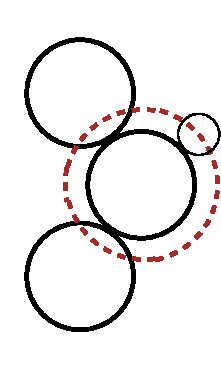
\includegraphics[width=0.5\linewidth]{rolling-ball.pdf}
	% TODO caption
	\caption{rolling-Ball}
	\label{fig:rolling-ball}
\end{figure}
